\chapter{Applications and Case Studies}
This chapter contains a number of case studies designed to deepen our understanding of \textsl{Python}.

\section{Solving Equations via Fixed-Point Algorithms}
\blue{Fixed-Point iterations} are very important, both in computer science and in mathematics.  As a first
example, we show how to solve an equation via a fixed point iteration.  Suppose we want to solve the equation  
\\[0.2cm]
\hspace*{1.3cm} $x = \cos(x)$. \\[0.2cm]
Here, $x$ is a real number that we seek to compute.  Figure \ref{fig:xEqualsCosX.pdf} on page
\pageref{fig:xEqualsCosX.pdf} shows the graphs of the two functions  
\\[0.2cm]
\hspace*{1.3cm}
$y = x$  \quad and \quad $y = \cos(x)$.
\\[0.2cm]
Since the graphs of these functions intersect, it is obvious that there exists a value $x$ such that $x = \cos(x)$. 
Furthermore, from Figure \ref{fig:xEqualsCosX.pdf} it is obvious that this value of $x$ is bigger than $0.6$
and less than $0.8$. 

\begin{figure}[!ht]
  \hspace*{-3.0cm}
  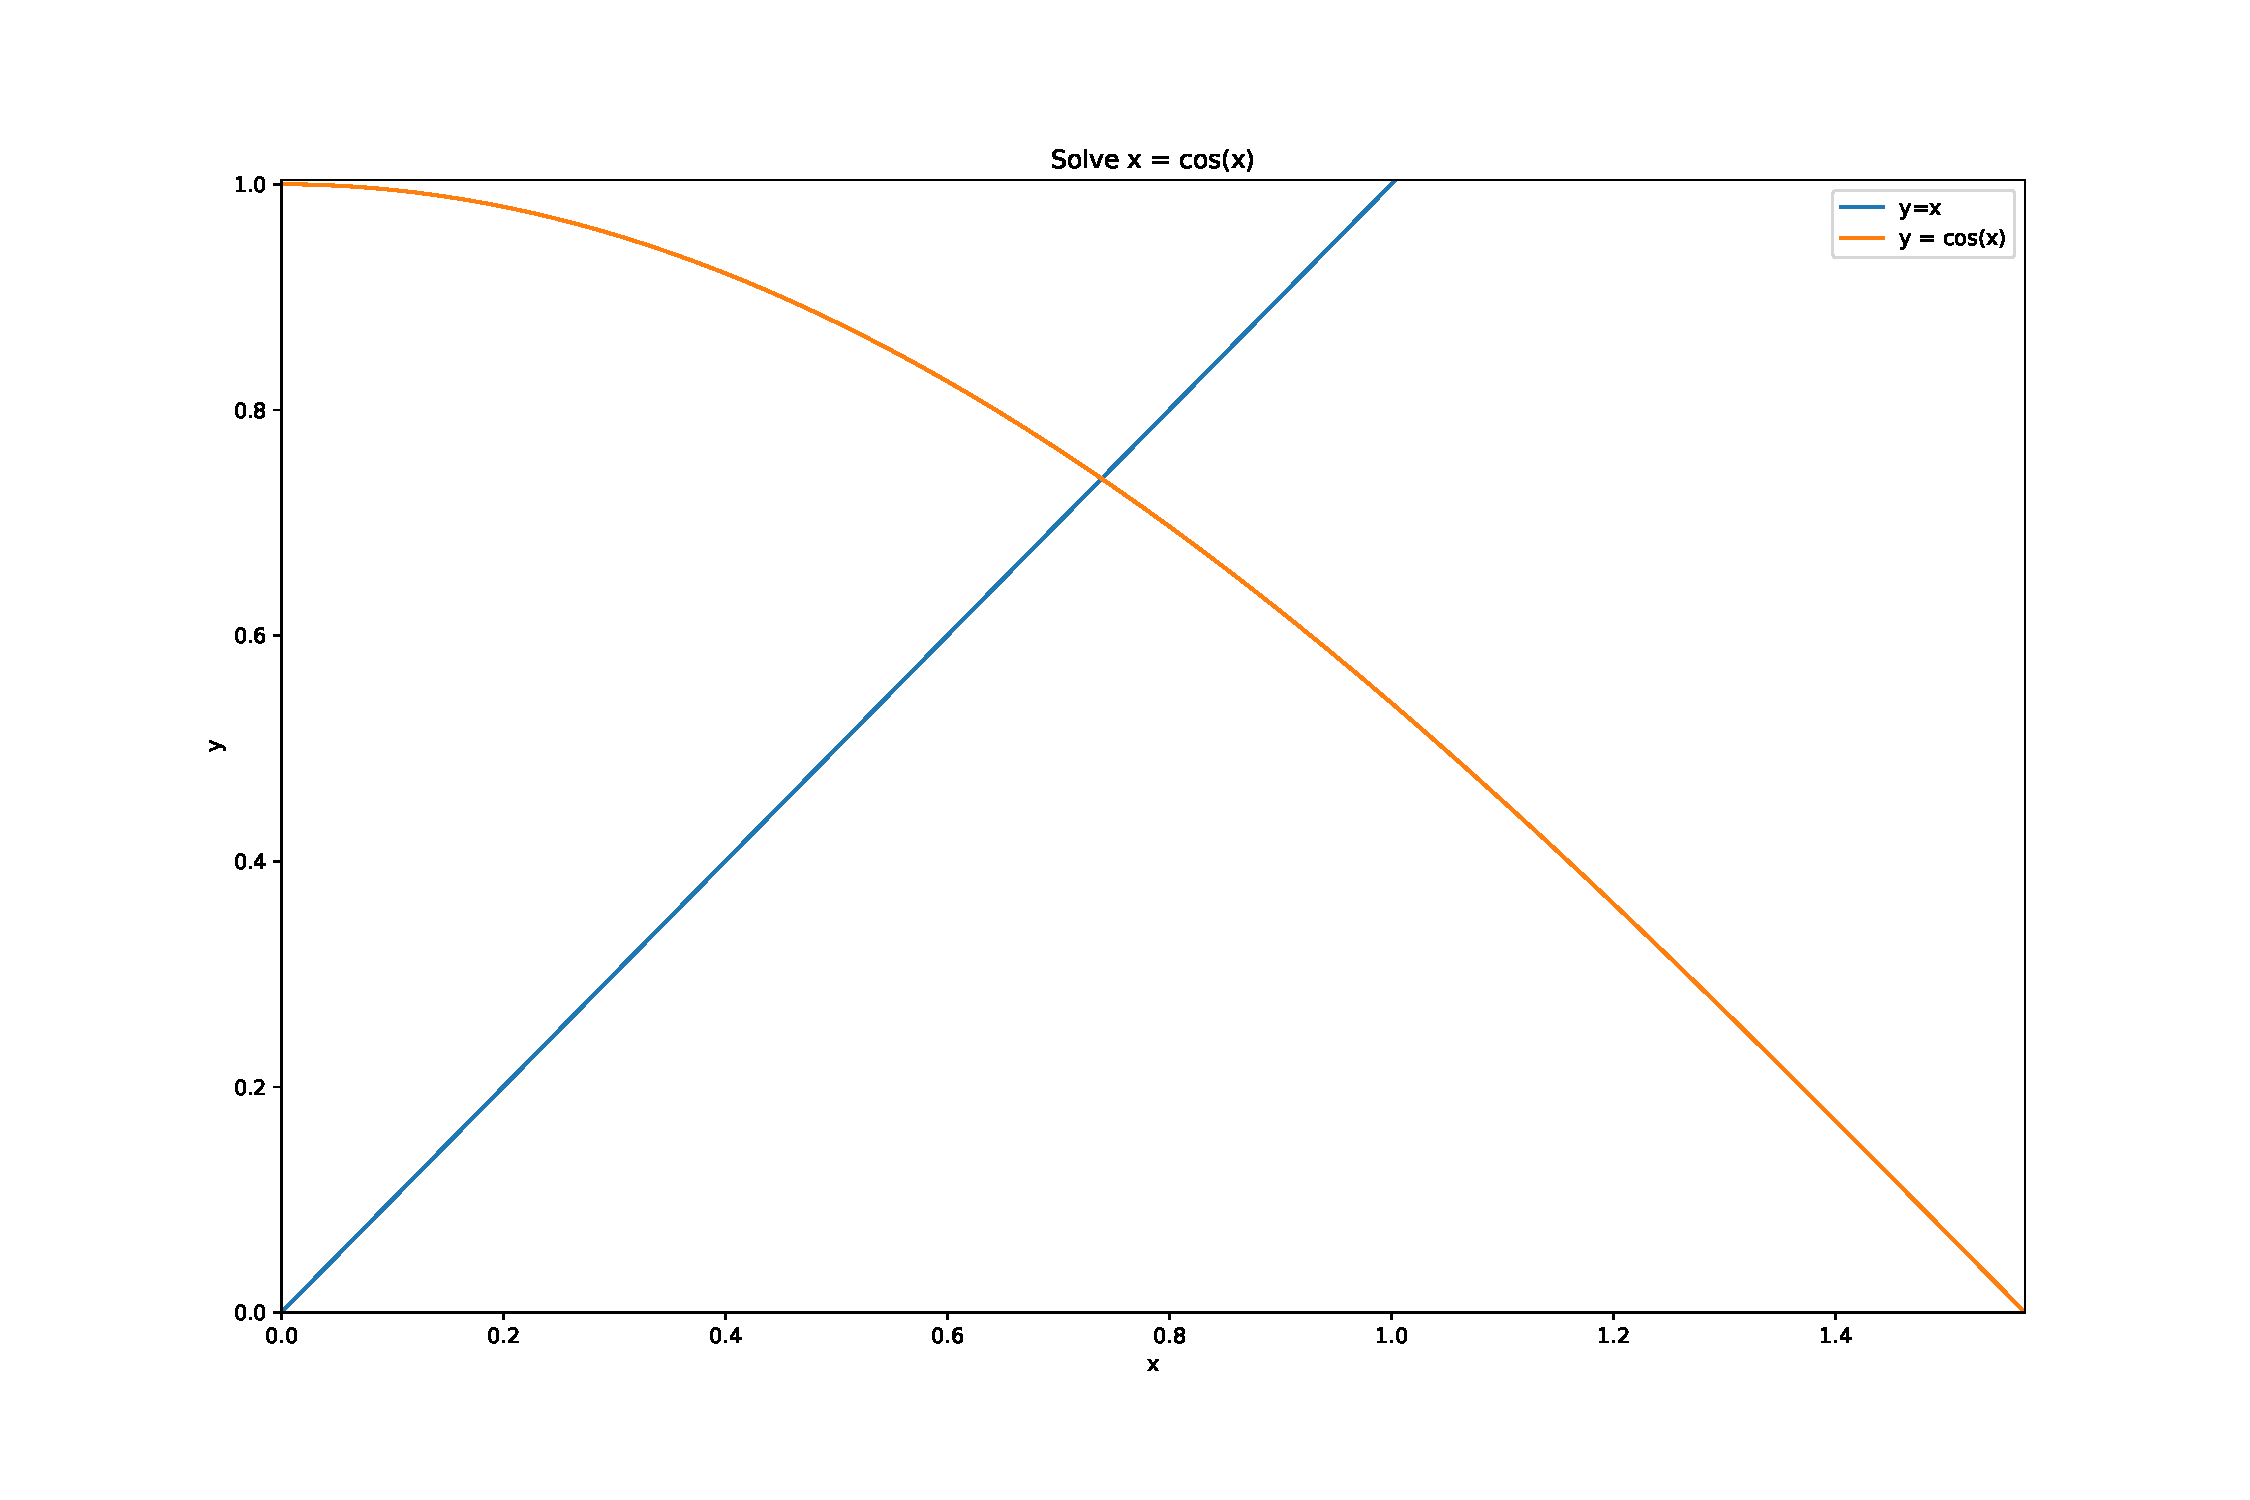
\epsfig{file=Figures/xEqualsCosX.pdf,scale=0.6}

  \caption{The functions $y = x$ and $y = cos(x)$.}
  \label{fig:xEqualsCosX.pdf}
\end{figure}



A simple approach that lets us compute the exact value of $x$ is to use a
\href{https://en.wikipedia.org/wiki/Fixed-point_iteration}{fixed-point iteration}.  To this end, we
define the sequence $\bigl(x_n\bigr)_{n\in\mathbb{N}}$ inductively as follows:
\\[0.2cm]
\hspace*{1.3cm} 
$x_0 = 0$ \quad and \quad $x_{n+1} = \mathtt{cos}(x_n)$ \quad for all $n \in \mathbb{N}$. 
\\[0.2cm]
With the help of the 
\href{https://en.wikipedia.org/wiki/Banach_fixed-point_theorem}{Banach fixed-point theorem}\footnote{
  The Banach fixed-point theorem is discussed in the lecture on
  \href{https://en.wikipedia.org/wiki/Differential_calculus}{differential calculus}.  This lecture is part of the
  second semester.
}
it can be shown that this sequence converges to a solution of the equation $x = \cos(x)$, i.e.~if we define
\\[0.2cm]
\hspace*{1.3cm}
$\bar{x} = \lim\limits_{n\rightarrow\infty} x_n$,
\\[0.2cm]
then we have
\\[0.2cm]
\hspace*{1.3cm}
$\cos\bigl(\bar{x}\bigr) = \bar{x}$.
\\[0.2cm]
Figure \ref{fig:solve.py} on page \pageref{fig:solve.py} shows the program
\href{https://github.com/karlstroetmann/Logik/blob/master/Python/solve.py}{\texttt{solve.py}}
that uses this approach to solve the equation $x = \cos(x)$.


\begin{figure}[!ht]
  \centering
\begin{Verbatim}[ frame         = lines, 
                  framesep      = 0.3cm, 
                  labelposition = bottomline,
                  numbers       = left,
                  numbersep     = -0.2cm,
                  xleftmargin   = 0.8cm,
                  xrightmargin  = 0.8cm,
                ]
    import math
    
    x     = 1.0
    old_x = 0.0
    i     = 1
    while abs(x - old_x) >= 4.0E-16:
        old_x = x
        x = math.cos(x)
        print(f'{i} : {x}')
        i += 1
\end{Verbatim} 
\vspace*{-0.3cm}
\caption{Solving the equation $x = \cos(x)$ via fixed-point iteration.}  \label{fig:solve.py}
\end{figure} %\$

In this program, the iteration stops as soon as the difference between the variables \texttt{x} and 
\texttt{old\_x} is less that $4 \cdot 10^{-16}$.  Here, \texttt{x} corresponds to $x_{n+1}$, while \texttt{old\_x}
corresponds to $x_n$.  Once the values of $x_{n+1}$ and $x_n$ are sufficiently close, the execution of the \texttt{while} loop
terminates.
\href{https://github.com/karlstroetmann/Logik/blob/master/Python/Fixed-Point-Iteration.ipynb}{Fixed-Point-Iteration.ipynb}
shows a \textsl{Jupyter} notebook that implements fixed point iteration.


\begin{figure}[!ht]
\centering
\begin{Verbatim}[ frame         = lines, 
                  framesep      = 0.3cm, 
                  firstnumber   = 1,
                  labelposition = bottomline,
                  numbers       = left,
                  numbersep     = -0.2cm,
                  xleftmargin   = 0.8cm,
                  xrightmargin  = 0.8cm,
                ]
    from math import cos
    
    def solve(f, x0):
        """
        Solve the equation f(x) = x using a fixed point iteration.
        x0 is the start value.
        """
        x = x0
        for n in range(10000):  # at most 10000 iterations
            oldX = x;
            x    = f(x);
            if abs(x - oldX) < 1.0e-15: 
                return x;
    
    print("solution to x = cos(x): ", solve(cos, 0));
    print("solution to x = 1/(1+x):", solve(lambda x: 1/(1+x), 0));
\end{Verbatim}
\vspace*{-0.3cm}
\caption{A generic implementation of the fixed-point algorithm.}
\label{fig:fixpoint.py}
\end{figure}

Figure \ref{fig:fixpoint.py} on page \pageref{fig:fixpoint.py} shows the program
\href{https://github.com/karlstroetmann/Logik/blob/master/Python/fixpoint.py}{\texttt{fixpoint.py}}.
In this program we have implemented a function \texttt{solve} that takes two arguments.
\begin{enumerate}
\item \texttt{f} is a unary function.  The purpose of the \texttt{solve} is to compute the solution of the equation
      \\[0.2cm]
      \hspace*{1.3cm}
      $f(x) = x$.
      \\[0.2cm]
      This equation is solved with the help of a fixed-point algorithm.
\item \texttt{x0} is used as the initial value for the fixed-point iteration.
\end{enumerate}
Line 11 calls \texttt{solve} to compute the solution of the equation $x = \cos(x)$.
Line 12 solves the equation 
\\[0.2cm]
\hspace*{1.3cm}
$\ds x = \bruch{1}{1+x}$. 
\\[0.2cm]
This equation is equivalent to the quadratic equation $x^2 + x = 1$.  Note that we have defined the function
 $\ds x \mapsto \frac{1}{1+x}$ via the expression
 \\[0.2cm]
\hspace*{1.3cm}
\texttt{lambda x: 1/(1+x)}.
\\[0.2cm]
This expression is called an \blue{anonymous function} since we haven't given a name to the function.  

\remarkEng
The function \texttt{solve} is only able to solve the equation $f(x) = x$ if the function $f$ is a 
\href{https://en.wikipedia.org/wiki/Contraction_mapping}{contraction mapping}.  A function 
$f:\mathbb{R} \rightarrow \mathbb{R}$
is called a \blue{contraction mapping} iff 
\\[0.2cm]
\hspace*{1.3cm}
$|f(x) - f(y)| < |x - y|$ \quad for all $x,y \in \mathbb{R}$.
\\[0.2cm]
This notion will be discussed in more detail in the lecture on 
\href{https://github.com/karlstroetmann/Analysis/blob/master/Script/analysis.pdf}{analysis} in the second
semester. \eox  

\section{Case Study: Computation of Poker Probabilities}
In this short section we are going to show how to compute probabilities for the
\href{https://en.wikipedia.org/wiki/Texas_hold_%27em}{\textsl{Texas Hold'em}} variation of 
\href{https://en.wikipedia.org/wiki/Poker}{poker}.   Texas Hold'em poker is played with a deck of 52
cards.  Every card has a \blue{value}.  This value is an element of the set
\\[0.2cm]
\hspace*{1.3cm} 
$\textsl{Values} = \{ 2, 3, 4, 5, 6, 7, 8, 9, 10, \textsl{Jack}, \textsl{Queen}, \textsl{King}, \textsl{Ace} \}$.
\\[0.2cm]
Furthermore, every card has a \blue{suit}.  This suit is an element of the set
\\[0.2cm]
\hspace*{1.3cm} 
$\textsl{Suits} = \{ \club, \mbox{$\color{red}{\heart}$}, \mbox{$\color{red}{\diamondsuit}$}, \spade \}$.
\\[0.2cm]
These suits are pronounced \blue{club}, \blue{heart}, \blue{diamond}, and \blue{spade}.
As a card is determined by its value and its suit, a card can be represented as a pair $\pair(v,s)$, where $v$
denotes the value while $s$ is the suit of the card.  Hence, the set of all cards can be represented as the set
\\[0.2cm]
\hspace*{1.3cm} 
$\textsl{Deck} = \bigl\{ \pair(v,s) \mid v \in \textsl{Values} \wedge \textsl{s} \in \textsl{Suits} \bigr\}$.
\\[0.2cm]
At the start of a game of Texas Hold'em, every player receives two cards.  These two cards are known
as the \blue{preflop} or the \blue{hole}.  Next, there is a \blue{bidding phase} where players can bet on their
cards.   After this bidding phase, the dealer puts three cards open on the table.  These three cards are
known as \blue{flop}.  Let us assume that a player has been dealt the set of cards
\\[0.2cm]
\hspace*{1.3cm}
$\{ \pair(3, \club), \pair(3, \spade) \}$.
\\[0.2cm]
This set of cards is known as a \blue{pocket pair}.  Then the player would like to know the probability
that the flop will contain another card with value $3$, as this would greatly increase her chance of
winning the game.  In order to compute this probability we have to compute the number of possible
flops that contain a card with the value $3$ and we have to divide this number by the number of all
possible flops:
\\[0.2cm]
\hspace*{1.3cm}
$\ds \frac{\;\mbox{number of flops containing a card with value $3$}\;}{\mbox{number of all possible flops}}$
\\[0.2cm]
The program
\href{https://github.com/karlstroetmann/Logik/blob/master/Python/poker-triple.py}{poker-triple.py}
shown in Figure \ref{fig:poker-triple.py} performs this computation.  We proceed to discuss this
program line by line.


\begin{figure}[!ht]
\centering
\begin{Verbatim}[ frame         = lines, 
                  framesep      = 0.3cm, 
                  labelposition = bottomline,
                  numbers       = left,
                  numbersep     = -0.2cm,
                  xleftmargin   = 0.0cm,
                  xrightmargin  = 0.0cm,
                ]
    Values = { "2", "3", "4", "5", "6", "7", "8", "9", "T", "J", "Q", "K", "A" } 
    Suits  = { "c", "h", "d", "s" }
    Deck   = { (v, s) for v in Values for s in Suits }
    Hole   = { ("3", "c"), ("3", "s") }
    Rest   = Deck - Hole
    Flops  = { (k1, k2, k3) for k1 in Rest for k2 in Rest for k3 in Rest 
                            if  len({ k1, k2, k3 }) == 3 
             }
    Trips  = { f for f in Flops if ("3", "d") in f or ("3", "h") in f }
    print(len(Trips) / len(Flops))
\end{Verbatim}
\vspace*{-0.3cm}
\caption{Computing a probability in poker.}
\label{fig:poker-triple.py}
\end{figure}

\begin{enumerate}
\item In line 1 the set \texttt{Values} is defined to be the set of all possible values that a card
      can take.  In defining this set we have made use of the following abbreviations:
      \begin{enumerate}
      \item ``\texttt{T}'' is short for ``\blue{Ten}'',
      \item ``\texttt{J}'' is short for ``\blue{Jack}'',
      \item ``\texttt{Q}'' is short for ``\blue{Queen}'',
      \item ``\texttt{K}'' is short for ``\blue{King}'', and
      \item ``\texttt{A}'' is short for ``\blue{Ace}''.
      \end{enumerate}
\item In line 2 the set \texttt{Suits} represents the possible suits of a card.  Here, we have used
      the following abbreviations:
      \begin{enumerate}
      \item ``\texttt{c}'' is short for $\club$, which is pronounced as \blue{club},
      \item ``\texttt{h}'' is short for \mbox{\color{red}{$\heart$}}, which is pronounced as \blue{heart}, 
      \item ``\texttt{d}'' is short for \mbox{\color{red}{$\diamondsuit$}}, which is pronounced as \blue{diamond}, and 
      \item ``\texttt{s}'' is short for $\spade$, which is pronounced as \blue{spade}. 
      \end{enumerate} 
\item Line 3 defines the set of all cards.  This set is stored as the variable \texttt{Deck}.  Every
      card is represented as a pair of the form $[v,s]$. Here, $v$ is the value of the card, while $s$ is its suit.
\item Line 4 defines the set \texttt{Hole}.  This set represents the two cards that have been given to our player.
\item The remaining cards are defined as the variable  \texttt{Rest} in line 5.
\item Line 6 computes the set of all possible flops.  Since the order of the cards in the flop does
      not matter, we use sets to represent these flops.  However, we have to take care that the flop
      does contain three \colorbox{amethyst}{different} cards.  Hence, we have to ensure that the three
      cards \texttt{k1}, \texttt{k2}, and \texttt{k3} that make up the flop satisfy the inequalities 
      \\[0.2cm]
      \hspace*{1.3cm}
      $\mathtt{k1} \not= \mathtt{k2}$, \quad $\mathtt{k1} \not= \mathtt{k3}$,  \quad and \quad $\mathtt{k2} \not= \mathtt{k3}$.
      \\[0.2cm]
      These inequalities are satisfied if and only if the set 
      $\{ \mathtt{k1}, \mathtt{k2}, \mathtt{k3} \}$ contains exactly three elements.  Hence, when
      choosing \texttt{k1}, \texttt{k2}, and \texttt{k3} we have to make sure that the condition
      \\[0.2cm]
      \hspace*{1.3cm}
      $\texttt{len}\bigl({\{ \mathtt{k1}, \mathtt{k2}, \mathtt{k3} \} \;\mathtt{==}\; 3 }\bigr)$
      \\[0.2cm]
      holds.
\item Line 9 computes the subset \texttt{Trips} of those flops that contain at least one card with a value of 3.
      As the 3 of clubs and the 3 of spades have already been dealt to our player, the only cards
      with value 3 that are left in the deck are the 3 of diamonds and the 3 of hearts.  Therefore, we are looking for
      those flops that contain one of these two cards.
\item Finally, the probability for obtaining another card with a value of 3 in the flop is computed as
      the ratio of the number of flops containing a card with a value of 3 to the number of all possible flops.
\end{enumerate}
When we run the program we see that the probability of improving a \blue{pocket pair} on the flop to \blue{trips} or better
is about  $11.8\%$.  A \textsl{Jupyter} notebook showcasing this computation outlined above can be fount at
\href{https://github.com/karlstroetmann/Logik/blob/master/Python/Poker.ipynb}{Poker.ipynb}.

\remarkEng
The method to compute probabilities that has been sketched above only works if the sets that have to
be computed are small enough to be retained in memory.  If this condition is
not satisfied we can use the \href{https://en.wikipedia.org/wiki/Monte_Carlo_method}{\emph{Monte Carlo method}} 
to compute the probabilities instead.  This method will be discussed in the lecture on 
\href{https://github.com/karlstroetmann/Algorithms/blob/master/Lecture-Notes/algorithms.pdf}{algorithms}.


\section{Finding a Path in a Graph}
In the following section, I will present an application that is more interesting since it is practically
relevant.  In order to prepare for this, we will now discuss the problem of finding a \blue{path} in a
\href{https://en.wikipedia.org/wiki/Directed_graph}{directed graph}. 
Abstractly, a graph consists of \blue{vertices} and \blue{edges} that connect these vertices.  In an application, the
vertices could be towns and villages, while the edges would be interpreted as streets connecting these
villages.  To simplify matters, let us assume for now that the vertices are given as natural numbers, while the
edges are represented as pairs of natural numbers.  Then, the graph can be represented as the set of its edges,
as the set of vertices is implicitly given once the edges are known.  To make things concrete, let us consider
an example.  In this case, the set of edges is called \texttt{R} and is defined as follows: 
\\[0.2cm]
\hspace*{1.3cm}
$\texttt{R}\; \mathtt{=}\; \bigl\{ \pair(1,2), \pair(2,3), \pair(1,3), \pair(2,4), \pair(4,5) \bigr\}$.
\\[0.2cm]
In this graph, the set of vertices is given as
\\[0.2cm]
\hspace*{1.3cm}
$\{ 1, 2, 3, 4, 5 \}$.
\\[0.2cm]
This graph is shown in Figure \ref{fig:graph0} on page \pageref{fig:graph0}.  You should note that the
connections between vertices that are given in this graph are \blue{unidirectional}:  While there is a connection from
vertex $1$ to vertex $2$, there is no connection from vertex $2$ to vertex $1$.

 
\begin{figure}[!ht]
  \centering
  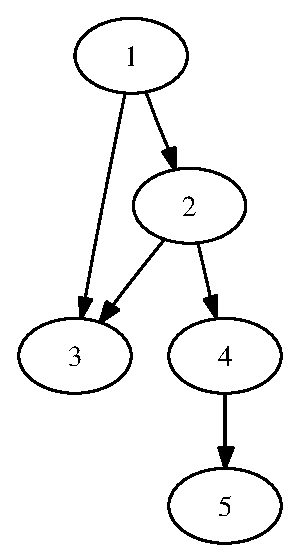
\epsfig{file=Figures/graph0,scale=0.6}

  \caption{A simple graph.}
  \label{fig:graph0}
\end{figure}



\noindent
The graph given by the relation \texttt{R} contains only the direct connections of vertices.  For example, in
the graph shown in Figure \ref{fig:graph0}, there is a direct connection from vertex $1$ to vertex $2$ and
another direct connection from vertex $2$ to vertex $4$.  Intuitively, vertex $4$ is reachable from vertex $1$,
since from vertex $1$ we can first reach vertex $2$ and from vertex $2$ we can then reach vertex $4$.  However,
there is is no direct connection between the vertices $1$ and $4$.  To make this more formal, define
a \blue{path} of a graph $R$ as a list of vertices
\\[0.2cm]
\hspace*{1.3cm}
$[x_1, x_2, \cdots, x_n]$ \quad such that \quad $\pair(x_i,x_{i+1}) \in R$ \quad for all $i=1,\cdots,n-1$.
\\[0.2cm]
In this case, the path $[x_1, x_2, \cdots, x_n]$ is written as
\\[0.2cm]
\hspace*{1.3cm}
$x_1 \mapsto x_2 \mapsto \cdots \mapsto x_n$
\\[0.2cm]
and has the \blue{length} $n-1$.  It is important to note that the length of a path
$[x_1,x_2,\cdots,x_n]$ is defined as the number of edges connecting the vertices and not as the
number of vertices appearing in the path.

Furthermore,  two vertices $a$ and $b$ are said to be \blue{connected} iff there exists a path
\\[0.2cm]
\hspace*{1.3cm}
$[x_1,\cdots,x_n]$ \quad such that \quad $a = x_1$ \quad and \quad $b = x_n$.
\\[0.2cm]
The goal of this section is to develop an algorithm that checks whether two vertices $a$ and $b$ are connected.
Furthermore, we want to be able to compute the corresponding path connecting the vertices $a$ and $b$.


\subsection{Computing the Transitive Closure of a Relation}
We have already noted that a graph can be represented as the set of its edges and hence as a \blue{binary relation}.
A \blue{binary relation} is defined as a set of pairs.  We also need the notion of a \blue{relational product}:
If $Q$ and $R$ are binary relations, then the \blue{relational product} $Q \circ R$ of $Q$ and $R$ is defined as
\\[0.2cm]
\hspace*{1.3cm}
$Q \circ R := \bigl\{ \pair(x, z) \bigm| \exists y:(\pair(x,y) \in Q \wedge \pair(y,z) \in R) \bigr\}$.
\\[0.2cm]
Furthermore, for any $n \in \mathbb{N}^*$ we can define the $n$-th power of the relation $R$ by induction.
\begin{enumerate}
\item[B.C.:] $n = 1$.

             $R^1 := R$
\item[I.S.:] $n \mapsto n+1$ 

             $R^{n+1} := R^n \circ R$.
\end{enumerate}
In order to decide whether there is a path connecting two vertices we have to compute the 
\href{https://en.wikipedia.org/wiki/Transitive_closure}{transitive closure} $R^+$ of a relation $R$.  
To understand this notion, we first need to define the concept of \blue{transitivity}:  A relation $R$ is
transitive if and only if the following holds:
\\[0.2cm]
\hspace*{1.3cm}
$\pair(x,y) \in T \wedge \pair(y, z) \in T \rightarrow \pair(x, z) \in T$ \quad for all $x,y,z$. 
\\[0.2cm]
Now the \blue{transitive closure} $R^+$ of a binary relation $R$ is the smallest relation $T$ such that the following
condition holds:
\begin{itemize}
\item $R$ is a subset of $T$, i.e. we have $R \subseteq T$.
\item $T$ is transitive.
\end{itemize}
The lecture on
\href{https://github.com/karlstroetmann/Lineare-Algebra/blob/master/Script/lineare-algebra.pdf}{Lineare Algebra} 
gives a prove that the transitive closure $R^+$ of a binary relation can be computed as follows:
\\[0.2cm]
\hspace*{1.3cm}
$R^+ = \bigcup\limits_{n=1}^{\infty} R^n = R^1 \cup R^2 \cup R^3 \cup \cdots$  
\\[0.2cm]
Initially, this formula might look intimidating as it suggests an infinite computation.
Fortunately, it turns out that we do not have to compute all powers of the form $R^n$.  Let me
explain the reason that allows us to cut the computation short.  
\begin{enumerate}
\item $R$ is the set of direct connections between two vertices.
\item $R^2$ is the same as $R \circ R$ and this relational product is defined as
      \\[0.2cm]
      \hspace*{1.3cm}
       $R \circ R = \bigl\{ \pair(x,z) \bigm| \exists y \colon(\pair(x,y) \in R \wedge \pair(y,z)) \in R \bigr\}$.
      \\[0.2cm]
      Hence, $R \circ R$ contains those pairs $\pair(x,z)$ that are connected via one intermediate vertex $y$,
      i.e.~there is a path of the form $x \mapsto y \mapsto z$ that connects $x$ and $z$.  This path
      has length 2.  In general, we can show by induction that $R^n$ connect those pairs that are
      connected by a path of length $n$.  The induction step of this proof runs as follows:
\item $R^{n+1}$ is defined as $R^n \circ R$ and therefore we have
      \\[0.2cm]
      \hspace*{1.3cm}
      $R^n \circ R = \{ \pair(x,z) \mid \exists y \colon \pair(x,y) \in R^n \wedge \pair(y,z) \in R \}$.
      \\[0.2cm]
      As $\pair(x,y) \in R^n$, the induction hypothesis guarantees that the vertices $x$ and $y$ are
      connected by a path of length $n$.  Hence, this 
      path has the form
      \\[0.2cm]
      \hspace*{1.3cm}
      $\underbrace{x \mapsto \cdots \mapsto y}_{\mbox{\scriptsize path of length $n$.}}$
      \\[0.2cm]
      Adding $x$ at the end of this path will produce the path
      \\[0.2cm]
      \hspace*{1.3cm}
      $x \mapsto \cdots \mapsto y \mapsto z$.
      \\[0.2cm]
      This path has a length of $n + 1$ and, furthermore, connects $x$ and $z$.  Hence $R^{n+1}$
      contains those pairs $\pair(x, z)$ that are connected by a path of length $n+1$.
\end{enumerate}
Now the important observation is the following. The set of all vertices is finite.  For the arguments sake, let
us assume there are $k$ different vertices.  But then every path that has a length of $k$ or greater must
contain at least one vertex that is visited more than once and hence this path is longer than necessary,
i.e.~there is a shorter path that connects the same vertices.  Therefore, for a finite graph with $k$ vertices,
the formula to compute the transitive closure can be simplified as follows:
\\[0.2cm]
\hspace*{1.3cm} 
$\ds R^+ = \bigcup\limits_{i=1}^{k-1} R^i$.
\\[0.2cm]
While we could use this formula as its stands, it is more efficient to use a \blue{fixed-point iteration} instead.
To this end, we prove that the transitive closure $R^+$ satisfies the following equation:
\begin{equation}
  \label{fixpunkt}
  R^+ = R \cup R^+ \circ R. 
\end{equation}
Let me remind you that the precedence of the operator $\circ$ 
is higher than the precedence of the operator $\cup$.  Therefore, the expression $R \cup R^+ \circ R$ is parenthesized
as $R \cup (R^+ \circ R)$.  Equation \ref{fixpunkt} can be proven algebraically.  We have:
\\[0.2cm]
\hspace*{1.3cm}
$
\begin{array}{cll}
    & R \cup R^+ \circ R \\[0.2cm]
  = & R \cup \Bigl(\bigcup\limits_{i=1}^{\infty} R^i \Bigr) \circ R \\[0.4cm]
  = & R \cup \bigl(R^1 \cup R^2 \cup R^3 \cup \cdots \bigr) \circ R \\[0.2cm]
  = & R \cup \bigl(R^1 \circ R \cup R^2 \circ R \cup R^3 \circ R \cup \cdots \bigr) \\[0.2cm]
  = & R \cup \bigl(R^2 \cup R^3 \cup  R^4 \cup \cdots \bigr)  \\[0.2cm]
  = & R^1 \cup \bigl(R^2 \cup R^3 \cup  R^4 \cup \cdots \bigr) \\[0.2cm]
  = & \bigcup\limits_{i=1}^{\infty} R^i \\[0.4cm]
  = & R^+.
\end{array}
$
\\[0.2cm]
Equation  \ref{fixpunkt} can now be used to compute $R^+$ via a fixed-point iteration.
To this end, let us define a sequence of relations $(T_n)_{n \in \mathbb{N}}$ by induction on $n$:
\begin{enumerate}
\item[I.A.] $n = 0$: 

            $T_0 = R$
\item[I.S.] $n \mapsto n+1$:

            $T_{n+1} = R \cup T_n \circ R $. 
\end{enumerate}
The relation  $T_n$ can be expressed via the relation $R$, we have
\begin{enumerate}
\item $T_0 = R$.
\item $T_1 = R \cup T_0 \circ R = R \cup R \circ R = R^1 \cup R^2$.
\item$\begin{array}[t]{lcl}
       T_2  & = & R \cup T_1 \circ R \\
            & = & R \cup (R^1 \cup R^2) \circ R \\
            & = & R^1 \cup R^2 \cup R^3. \\
       \end{array}
      $
\end{enumerate}
In general, we can show by induction that
\\[0.2cm]
\hspace*{1.3cm}
$T_n = \bigcup\limits_{i=1}^{n+1} R^i$
\\[0.2cm]
holds for all $n \in \mathbb{N}$.  The base case of this proof is immediate from the definition of $T_0$.
In the induction step we observe the following:
\\[0.2cm]
\hspace*{1.3cm}
$
 \begin{array}{lcll}
   T_{n+1} & = & \ds R \cup T_n \circ R & \mbox{(by definition)} \\[0.2cm]
           & = & \ds R \cup \biggl(\bigcup\limits_{i=1}^{n+1} R^i\biggr) \circ R &
                 \mbox{(by induction hypothesis)} \\[0.4cm]
           & = & \ds R \cup \left(R \cup \cdots \cup R^{n+1}\right) \circ R \\[0.2cm] 
           & = & \ds R^1 \cup R^2 \cup \cdots \cup R^{n+2}  &
                 \mbox{(by the distributivity of $\circ$ over $\cup$)} \\[0.2cm]
           & = & \ds \bigcup\limits_{i=1}^{n+2} R^i & \Box 
   \end{array}
$
\\[0.2cm]
The sequence $(T_n)_{n\in\mathbb{N}}$ has another useful property:  It is 
\blue{monotonically increasing}.  In general, a sequence of sets $(X_n)_{n\in\mathbb{N}}$ is called
\blue{monotonically increasing} iff we have
\\[0.2cm]
\hspace*{1.3cm}
$\forall n \in \mathbb{N}: X_n \subseteq X_{n+1}$,
\\[0.2cm]
i.e.~the sets $X_n$ get bigger with growing index $n$.
The monotonicity of the sequence  $(T_n)_{n \in \mathbb{N}}$ is an immediate consequence of the equation
\\[0.2cm]
\hspace*{1.3cm}
$\ds T_n = \bigcup\limits_{i=1}^{n+1} R^i$ 
\\[0.2cm]
because we have:
\\[0.2cm]
\hspace*{1.3cm}
$
\begin{array}[t]{llcl}
                & \ds T_n \subseteq T_{n+1} \\[0.2cm]
\Leftrightarrow & \ds \bigcup\limits_{i=1}^{n+1} R^i \subseteq \bigcup\limits_{i=1}^{n+2} R^i \\[0.5cm]
\Leftrightarrow & \ds \bigcup\limits_{i=1}^{n+1} R^i \subseteq \bigcup\limits_{i=1}^{n+1} R^i \cup R^{n+2} \\
\end{array}
$
\\[0.2cm]
If the relation  $R$ is finite, then the transitive closure $R^+$ is finite, too.  The sets $T_n$ 
are all subsets of $R^+$ because we have
\\[0.2cm]
\hspace*{1.3cm}
$\ds T_n = \bigcup\limits_{i=1}^{n+1} R^i \subseteq \bigcup\limits_{i=1}^{\infty} R^i = R^+$ \quad for all $n \in \mathbb{N}$.
\\[0.2cm]
Hence the sets $T_n$ can not grow indefinitely.  Because of the monotonicity of the sequence 
$(T_n)_{n\in\mathbb{N}}$ it follows that there exists an index  $k \in \mathbb{N}$ such that the sets $T_n$ do
not grow any further once $n$ has reached $k$, i.e.~we have
\\[0.2cm]
\hspace*{1.3cm}
$\ds \forall n \in \mathbb{N}:( n \geq k \rightarrow T_n = T_k)$.
\\[0.2cm]
But this implies that
\\[0.2cm]
\hspace*{1.3cm}
$\ds T_n = \bigcup\limits_{i=1}^{n+1} R^i = \bigcup\limits_{i=1}^{\infty} R^i = R^+$ 
\quad holds for all $n \geq k$.
\\[0.2cm]
Therefore, the algorithm for computing  $R^+$ iterates the equation 
\\[0.2cm]
\hspace*{1.3cm}
$\ds T_{n+1} = R \cup T_n \circ R$
\\[0.2cm]
until the equation  $T_{n+1} = T_n$ is satisfied, since this implies that $T_n = R^+$.


\begin{figure}[!ht]
  \centering
\begin{Verbatim}[ frame         = lines, 
                  framesep      = 0.3cm, 
                  labelposition = bottomline,
                  numbers       = left,
                  numbersep     = -0.2cm,
                  xleftmargin   = 0.8cm,
                  xrightmargin  = 0.8cm,
                ]
    def product(R1, R2):
        "Compute the relational product of R1 and R2."
        return { (x, z) for (x, y1) in R1 for (y2, z) in R2 if y1 == y2 }
    
    def transClosure(R):
        "Compute the transitive closure of the binary relation R."
        T = R
        while True:
            oldT = T
            T    = product(R,T).union(R)
            if T == oldT:
                return T
    
    R = { (1,2), (2,3), (1,3), (2,4), (4,5) }
    print( "R  = ", R );
    print( "Computing the transitive closure of R:" );
    T = transClosure(R);
    print( "R+ = ", T );
\end{Verbatim} 
\vspace*{-0.3cm}
\caption{Computing the transitive closure.}  
\label{fig:transitive-closure.py}
\end{figure} %\$

\noindent
The program 
\href{https://github.com/karlstroetmann/Logik/blob/master/Python/transitive-closure.py}{\texttt{transitive-closure.py}}
that is shown in Figure
\ref{fig:transitive-closure.py} on page \pageref{fig:transitive-closure.py} shows an implementation of this idea.
The program produces the following output:
\begin{verbatim}
    R  = {(1, 2), (1, 3), (4, 5), (2, 3), (2, 4)}
    Computing the transitive closure of R:
    R+ = {(1, 2), (1, 3), (4, 5), (1, 4), (1, 5), (2, 3), (2, 5), (2, 4)}
\end{verbatim}
The transitive closure $R^+$ of a relation $R$ has a very intuitive interpretation:
It contains all pairs $\pair(x,y)$ such that there is a path leading from 
$x$ to $y$.  
The function $\texttt{product}(R_1, R_2)$ computes the relational product $R_1\circ R_2$ 
according to the formula
\\[0.2cm]
\hspace*{1.3cm}
$R_1 \circ R_2 = \{ \langle x, z \rangle \mid \exists y:\bigl(\pair(x,y) \in R_1 \wedge \pair(y,z) \in R_2\bigr) \}$.


\subsection{Computing the Paths}
So far, given a graph represented by a relation $R$ and two vertices $x$ and $y$, we can only check
whether there is a path leading from $x$ to $y$, but we cannot compute this path.  In this
subsection we will extend the procedure \texttt{transClosure} so that it will also compute the
corresponding path.  The main idea is to extend the notion of a relational product to the notion of
a \blue{path product}, where a \blue{path product} is defined on sets of paths.  In order to do so,
we introduce three functions for tuples.
\begin{enumerate}
\item Given a tuple $T$, the function $\texttt{first}(T)$ returns the first element of $T$: 
      \\[0.2cm]
      \hspace*{1.3cm}
      $\texttt{first}\bigl(\langle x_1,\cdots,x_m\rangle\bigr) = x_1$.
\item Given a tuple $T$, the function $\texttt{last}(T)$ returns the last element of $T$: 
      \\[0.2cm]
      \hspace*{1.3cm}
      $\texttt{last}\bigl(\langle x_1,\cdots,x_m\rangle\bigl) = x_m$.
\item If $S = \langle x_1, \cdots, x_m\rangle$ and $T = \langle y_1, \cdots, y_n \rangle$ are two tuples  such that
      $\texttt{first}(S) = \texttt{last}(S)$, we define the \blue{join} $S \oplus T$ of $S$ and $T$ as \\[0.2cm]
      \hspace*{1.3cm}
      $S \oplus T = \langle x_1, \cdots, x_m, y_2, \cdots, y_n \rangle$.
\end{enumerate}
If $\mathcal{P}_1$ and $\mathcal{P}_2$ are sets of tuples representing paths, we define the \blue{path product} of
$\mathcal{P}_1$ and $\mathcal{P}_2$ as follows: \\[0.2cm]
\hspace*{1.3cm} 
$\mathcal{P}_1 \bullet \mathcal{P}_2 = 
\bigl\{\; T_1 \oplus T_2 \mid T_1 \in \mathcal{P}_1 \wedge T_2 \in \mathcal{P}_2 \wedge \texttt{last}(T_1) = \texttt{first}(T_2) \;\bigr\}
$.

\begin{figure}[!ht]
  \centering
\begin{Verbatim}[ frame         = lines, 
                  framesep      = 0.3cm, 
                  labelposition = bottomline,
                  numbers       = left,
                  numbersep     = -0.2cm,
                  xleftmargin   = 0.8cm,
                  xrightmargin  = 0.8cm,
                ]
    def findPaths(R):
        P = R;
        while True:
            oldP = P
            P    = R.union(pathProduct(P, R))
            print(P)
            if P == oldP:
                return P

    def pathProduct(P, Q):
        return { join(S, T) for S in P for T in Q if S[-1] == T[0] }
    
    def join(S, T):
        return S + T[1:]
    
    R = { (1,2), (2,3), (1,3), (2,4), (4,5) }
    print("R = ", R)
    print("Computing all paths:" )
    P = findPaths(R)
    print("P = ", P)
\end{Verbatim} 
\vspace*{-0.3cm}
\caption{Computing all connections.}  \label{fig:path.py}
\end{figure} %\$

\begin{figure}[!ht]
  \centering
  \vspace*{-9cm}

  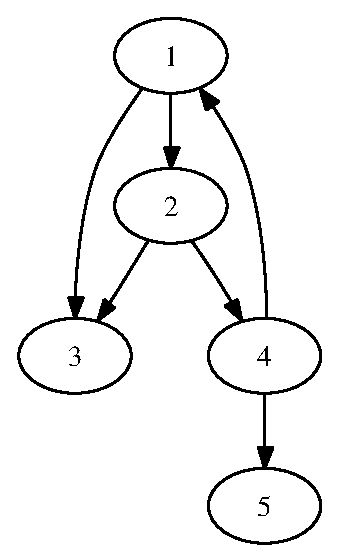
\epsfig{file=Figures/graph-zykl,scale=0.5}
  \vspace*{-1cm}

  \caption{A graph with a cycle.}
  \label{fig:graph-zykl}
\end{figure}

Using the notion of a \blue{path product} we are able to extend the program shown in Figure
\ref{fig:transitive-closure.py} such that it computes all paths between two vertices.
The resulting program
\href{https://github.com/karlstroetmann/Logik/blob/master/Python/path.py}{\texttt{path.py}}
is shown in Figure \ref{fig:path.py} on page \pageref{fig:path.py}.
Unfortunately, the program does not work any more if the graph is \blue{cyclic}.  A graph is defined
to be \blue{cyclic} if there is a path of length greater than $1$ that starts and ends at the same
vertex.  This path is then called a \blue{cycle}.
Figure \ref{fig:graph-zykl} on page \pageref{fig:graph-zykl} shows a cyclic graph.  This graph is
cyclic because it contains the path
\\[0.2cm]
\hspace*{1.3cm}
$\langle 1, 2, 4, 1 \rangle$
\\[0.2cm]
and this path is a cycle.
The problem with this graph is that it contains an infinite number of paths that connect the vertex
1 with the vertex 2: \\[0.2cm]
\hspace*{1.3cm}
$\langle 1, 2 \rangle$, $\langle 1, 2, 4, 1, 2 \rangle$, 
$\langle 1, 2, 4, 1, 2, 4, 1, 2 \rangle$, 
$\langle 1, 2, 4, 1, 2, 4, 1, 2, 4, 1, 2 \rangle$, $\cdots$
\\[0.2cm]
Of course, there is no point in computing a path that visits a vertex more than once as these paths
contain cycles.  Our goal is to eliminate all those paths that contain cycles.


\begin{figure}[!ht]
  \centering
\begin{Verbatim}[ numbers       = left,
                  numbersep     = -0.2cm,
                  frame         = lines, 
                  framesep      = 0.3cm, 
                  labelposition = bottomline,
                  xleftmargin   = 0.0cm,
                  xrightmargin  = 0.0cm,
                ]
    def pathProduct(P, Q):
        return { join(S, T) for S in P for T in Q
                            if S[-1] == T[0] and noCycle(S, T)
               }
    
    def noCycle(T1, T2):
        return len({ x for x in T1 }.intersection({ x for x in T2 })) == 1
\end{Verbatim} 
\vspace*{-0.3cm}
\caption{Computing the connections in a cyclic graph.}  
\label{fig:path-cyclic.py}
\end{figure} %\$

Figure \ref{fig:path-cyclic.py} on page shows how the implementation of the function
\texttt{pathProduct} has to be changed so that the resulting program
\href{https://github.com/karlstroetmann/Logik/blob/master/Python/path-cyclic.py}{\texttt{path-cyclic.py}}
works also for cyclic graphs. 
\begin{enumerate}
\item In line 2 and 3, we compute only those paths that are not cyclic.
\item Line 6 defines a function \texttt{noCycle} that tests, whether the join  $\texttt{T1} \oplus \texttt{T2}$ is cyclic.  The join
      of \texttt{T1} and \texttt{T2} is cyclic iff the tuples \texttt{T1} and \texttt{T2} have more
      than one common element.  The tuples \texttt{T1} and \texttt{T2} will always have at least one common element, as we join
      these tuples only if the last element of \texttt{T1} is equal to the first element of  \texttt{T2}.
      If there would be an another vertex common to both \texttt{T1} and \texttt{T2}, then the path
      $\texttt{T1} \oplus \texttt{T2}$ would be cyclic.
\end{enumerate}

In general, we are not really interested to compute all possible paths between two given vertices
\texttt{x} and \texttt{y}.  Instead, we just want to compute the shortest path leading from \texttt{x} to \texttt{y}.
Figure \ref{fig:find_path.py} on page \pageref{fig:find_path.py} shows the procedure \texttt{reachable}. 
This procedure takes three arguments:
\begin{enumerate}
\item \texttt{start} and \texttt{goal} are vertices of a graph.
\item \texttt{R} is a binary relation representing a directed graph.
\end{enumerate}
The call  \texttt{reachable(start, goal, R)} checks whether \texttt{start} and \texttt{goal} are connected and, furthermore,
computes the shortest path from \texttt{start} to \texttt{goal}, provided such a path exists.
The complete program can be found in the file
\href{https://github.com/karlstroetmann/Logik/blob/master/Python/find\_path.py}{\texttt{find\_path.py}}.
Next, we discuss the implementation of the procedure  \texttt{reachable}.
\begin{enumerate}
\item Line 2 initializes the set \texttt{P}.  After $n$ iterations, this set will contain all paths
      that start with the vertex \texttt{start} and that have a length of at most $n$.

      Initially, there is just the trivial path $\langle\texttt{start}\rangle$ that starts with vertex
      \texttt{start} and has length $0$.
\item Line 5 tries to extend all previously computed paths by one step.
      If we are lucky, the set \texttt{P} is increased in this step.
\item Line 6 selects all those paths from the set \texttt{P} that lead to the vertex \texttt{goal}.
      These paths are stored in the set \texttt{Found}.
\item Line 7 checks whether we have indeed found a path ending at \texttt{goal}.  This is the case if
      the set \texttt{Found} is not empty.  
      In this case, we return any of these paths.
\item If we have not yet found the vertex \texttt{goal} and, furthermore, we have not been able to find
      any new paths during this iteration,  the procedure returns in line 10.
      As the \texttt{return} statement in line 11 does not return a value, the procedure will
      instead return the value \texttt{None}.
\end{enumerate}
The procedure call \texttt{reachable(start,goal R)} will compute the \textbf{shortest} path connecting
\texttt{start} and \texttt{goal} because it computes path with increasing length.  The first iteration
computes all paths starting in \texttt{start} that have a length of at most 1, the second iteration
computes all paths starting in \texttt{start} that have a length of at most 2, and in general the $n$-th
iteration computes all paths starting in \texttt{start} that have a length of at most $n$.  Hence, if
there is a path of length $n$, then this path will be found in the $n$-iteration unless a shorter path has
already been found in a previous iteration.  

\remarkEng
The algorithm described above is known as 
\href{https://en.wikipedia.org/wiki/Breadth-first_search}{breadth first search}. \eox 

\begin{figure}[!ht]
  \centering
\begin{Verbatim}[ frame         = lines, 
                  framesep      = 0.3cm, 
                  labelposition = bottomline,
                  numbers       = left,
                  numbersep     = -0.2cm,
                  xleftmargin   = 0.8cm,
                  xrightmargin  = 0.8cm,
                ]
    def reachable(start, goal, R):
        P = { (start,) }
        while True:
            oldP  = P
            P     = P.union(path_product(P, R))
            Found = { T for T in P if T[-1] == goal }
            if Found != set({}):
                return Found.pop()
            if P == oldP:
                return
                
    def path_product(P, R):
        return set( add(T1, T2) for T1 in P for T2 in R
                             if T1[-1] == T2[0] and noCycle(T1, T2)
                  )
    
    def noCycle(T1, T2):
        return len(set(T1).intersection(set(T2))) == 1
    
    def add(T, P):
        return T + (P[-1],)
\end{Verbatim} 
\vspace*{-0.3cm}
\caption{Finding the shortest path between two vertices.}  
\label{fig:find_path.py}
\end{figure}

\subsection{The Wolf, the Goat, and the Cabbage}
Next, we present an application of the theory developed so far.  We solve a problem that has puzzled
the greatest agricultural economists for centuries.  The puzzle we want to solve is known as the 
\href{http://jeux.lulu.pagesperso-orange.fr/html/anglais/loupChe/loupChe1.htm}{wolf-goat-cabbage puzzle}:  
\vspace*{0.3cm}

\begin{minipage}[c]{14cm}
{\sl
An agricultural economist has to sell a wolf, a goat, and a cabbage on a market place.  In order to
reach the market place, she has to cross a river.  The boat that she can use is so small that it can
only accommodate either the goat, the wolf, or the cabbage in addition to the agricultural economist.
Now if the agricultural economist leaves the wolf alone with the goat, the wolf will eat the goat.
If, instead, the agricultural economist leaves the goat with the cabbage, the goat will eat the cabbage.
Is it possible for the agricultural economist to develop a schedule that allows her to cross the river
without either the goat or the cabbage being eaten?
}
\end{minipage}
\vspace*{0.3cm}

\noindent
In order to compute a schedule, we first have to model the problem.  The various \blue{states} of the problem will
be regarded as \blue{vertices} of a graph and this graph will be represented as a binary relation.
To this end we define the set
\begin{verbatim}
  All = {'farmer', 'wolf, 'goat', 'cabbage'}
\end{verbatim}
Every node will be represented as a subset \texttt{S} of the set \texttt{All}.  The idea is that the set \texttt{S}
specifies those objects that are on the left side of the river.  We assume that initially the farmer
is on the left side of the river. 
Therefore, the set of all possible states can be defined as the set
\begin{verbatim}
  States = {S for S in power(All) if not problem(S) and not problem(All-S)}
\end{verbatim}
Here, we have used the procedure \texttt{problem} to check whether a given set \texttt{S} has a problem. 
Note that since \texttt{S} is the set of objects on the left side, the expression $\texttt{All-S}$
computes the set of objects on the right side of the river.

Next, a set \texttt{S} of objects has a problem if both of the following conditions
are satisfied:
\begin{enumerate}
\item The farmer is not an element of \texttt{S} and
\item either \texttt{S} contains both the goat and the cabbage or \texttt{S} contains both the wolf and the goat.
\end{enumerate}
Therefore, we can implement the function \texttt{problem} as follows:
\begin{verbatim}
  def problem(S):
      return ("farmer" not in S) and             \
             (("goat" in S and "cabbage" in S) or   # goat eats cabbage
              ("wolf" in S and "goat"    in S)   )  # wolf eats goat
\end{verbatim}
We proceed to compute the relation \texttt{R} that contains all possible transitions between
different states.  We will compute \texttt{R} using the formula:
\\[0.2cm]
\hspace*{0.75cm}
\texttt{R = R1 + R2;}
\\[0.2cm]
Here \texttt{R1} describes the transitions that result from the farmer crossing the river from left
to right, while \texttt{R2} describes the transitions that result from the farmer crossing the river
from right to left.  We can define the relation \texttt{R1} as follows:
\begin{verbatim}
  R1 = { (S, S-B) for S in States for B in power(S)
                  if S-B in States and 'farmer' in B and len(B) <= 2
       }
\end{verbatim}
Let us explain this definition in detail:
\begin{enumerate}
\item Initially, \texttt{S} is the set of objects on the left side of the river.  Hence, \texttt{S}
      is an element of the set of all states that we have defined as \texttt{P}.
\item \texttt{B} is the set of objects that are put into the boat and that do cross the river.  Of
      course, for an object to go into the boat is has to be on the left side of the river to begin
      with.  Therefore, \texttt{B} is a subset of \texttt{S} and hence an element of the power set
      of \texttt{S}. 
\item Then  \texttt{S-B} is the set of objects that are left on the left side of the river after
      the boat has crossed.  Of course, the new state \texttt{S-B} has to be a state that does not
      have a problem.  Therefore, we check that \texttt{S-B} is an element of \texttt{States}.
\item Furthermore, the farmer has to be inside the boat.  This explains the condition 
      \\[0.2cm]
      \hspace*{1.3cm}
      \texttt{\symbol{39}farmer\symbol{39} in B}.
\item Finally, the boat can only have two passengers.  Therefore, we have added the condition
      \\[0.2cm]
      \hspace*{1.3cm}
      \texttt{len(B) <= 2}.
\end{enumerate}
Next, we have to define the relation \texttt{R2}.  However, as crossing the river from right to left
is just the reverse of crossing the river from left to right, \texttt{R2} is just the \blue{inverse} of
\texttt{R1}.   Hence we define:
\begin{verbatim}
  R2 = { (S2, S1) for (S1, S2) in R1 }
\end{verbatim}
Next, the relation \texttt{R} is the union of \texttt{R1} and \texttt{R2}:
\begin{verbatim}
  R = R1.union(R2)
\end{verbatim}
Finally, the start state has all objects on the left side.  Therefore, we have
\begin{verbatim}
  start = All
\end{verbatim}
In the end, all objects have to be on the right side of the river.  That means that nothing is left
on the left side.  Therefore, we define
\begin{verbatim}
  goal = {}
\end{verbatim}


\begin{figure}[h]
  \centering

  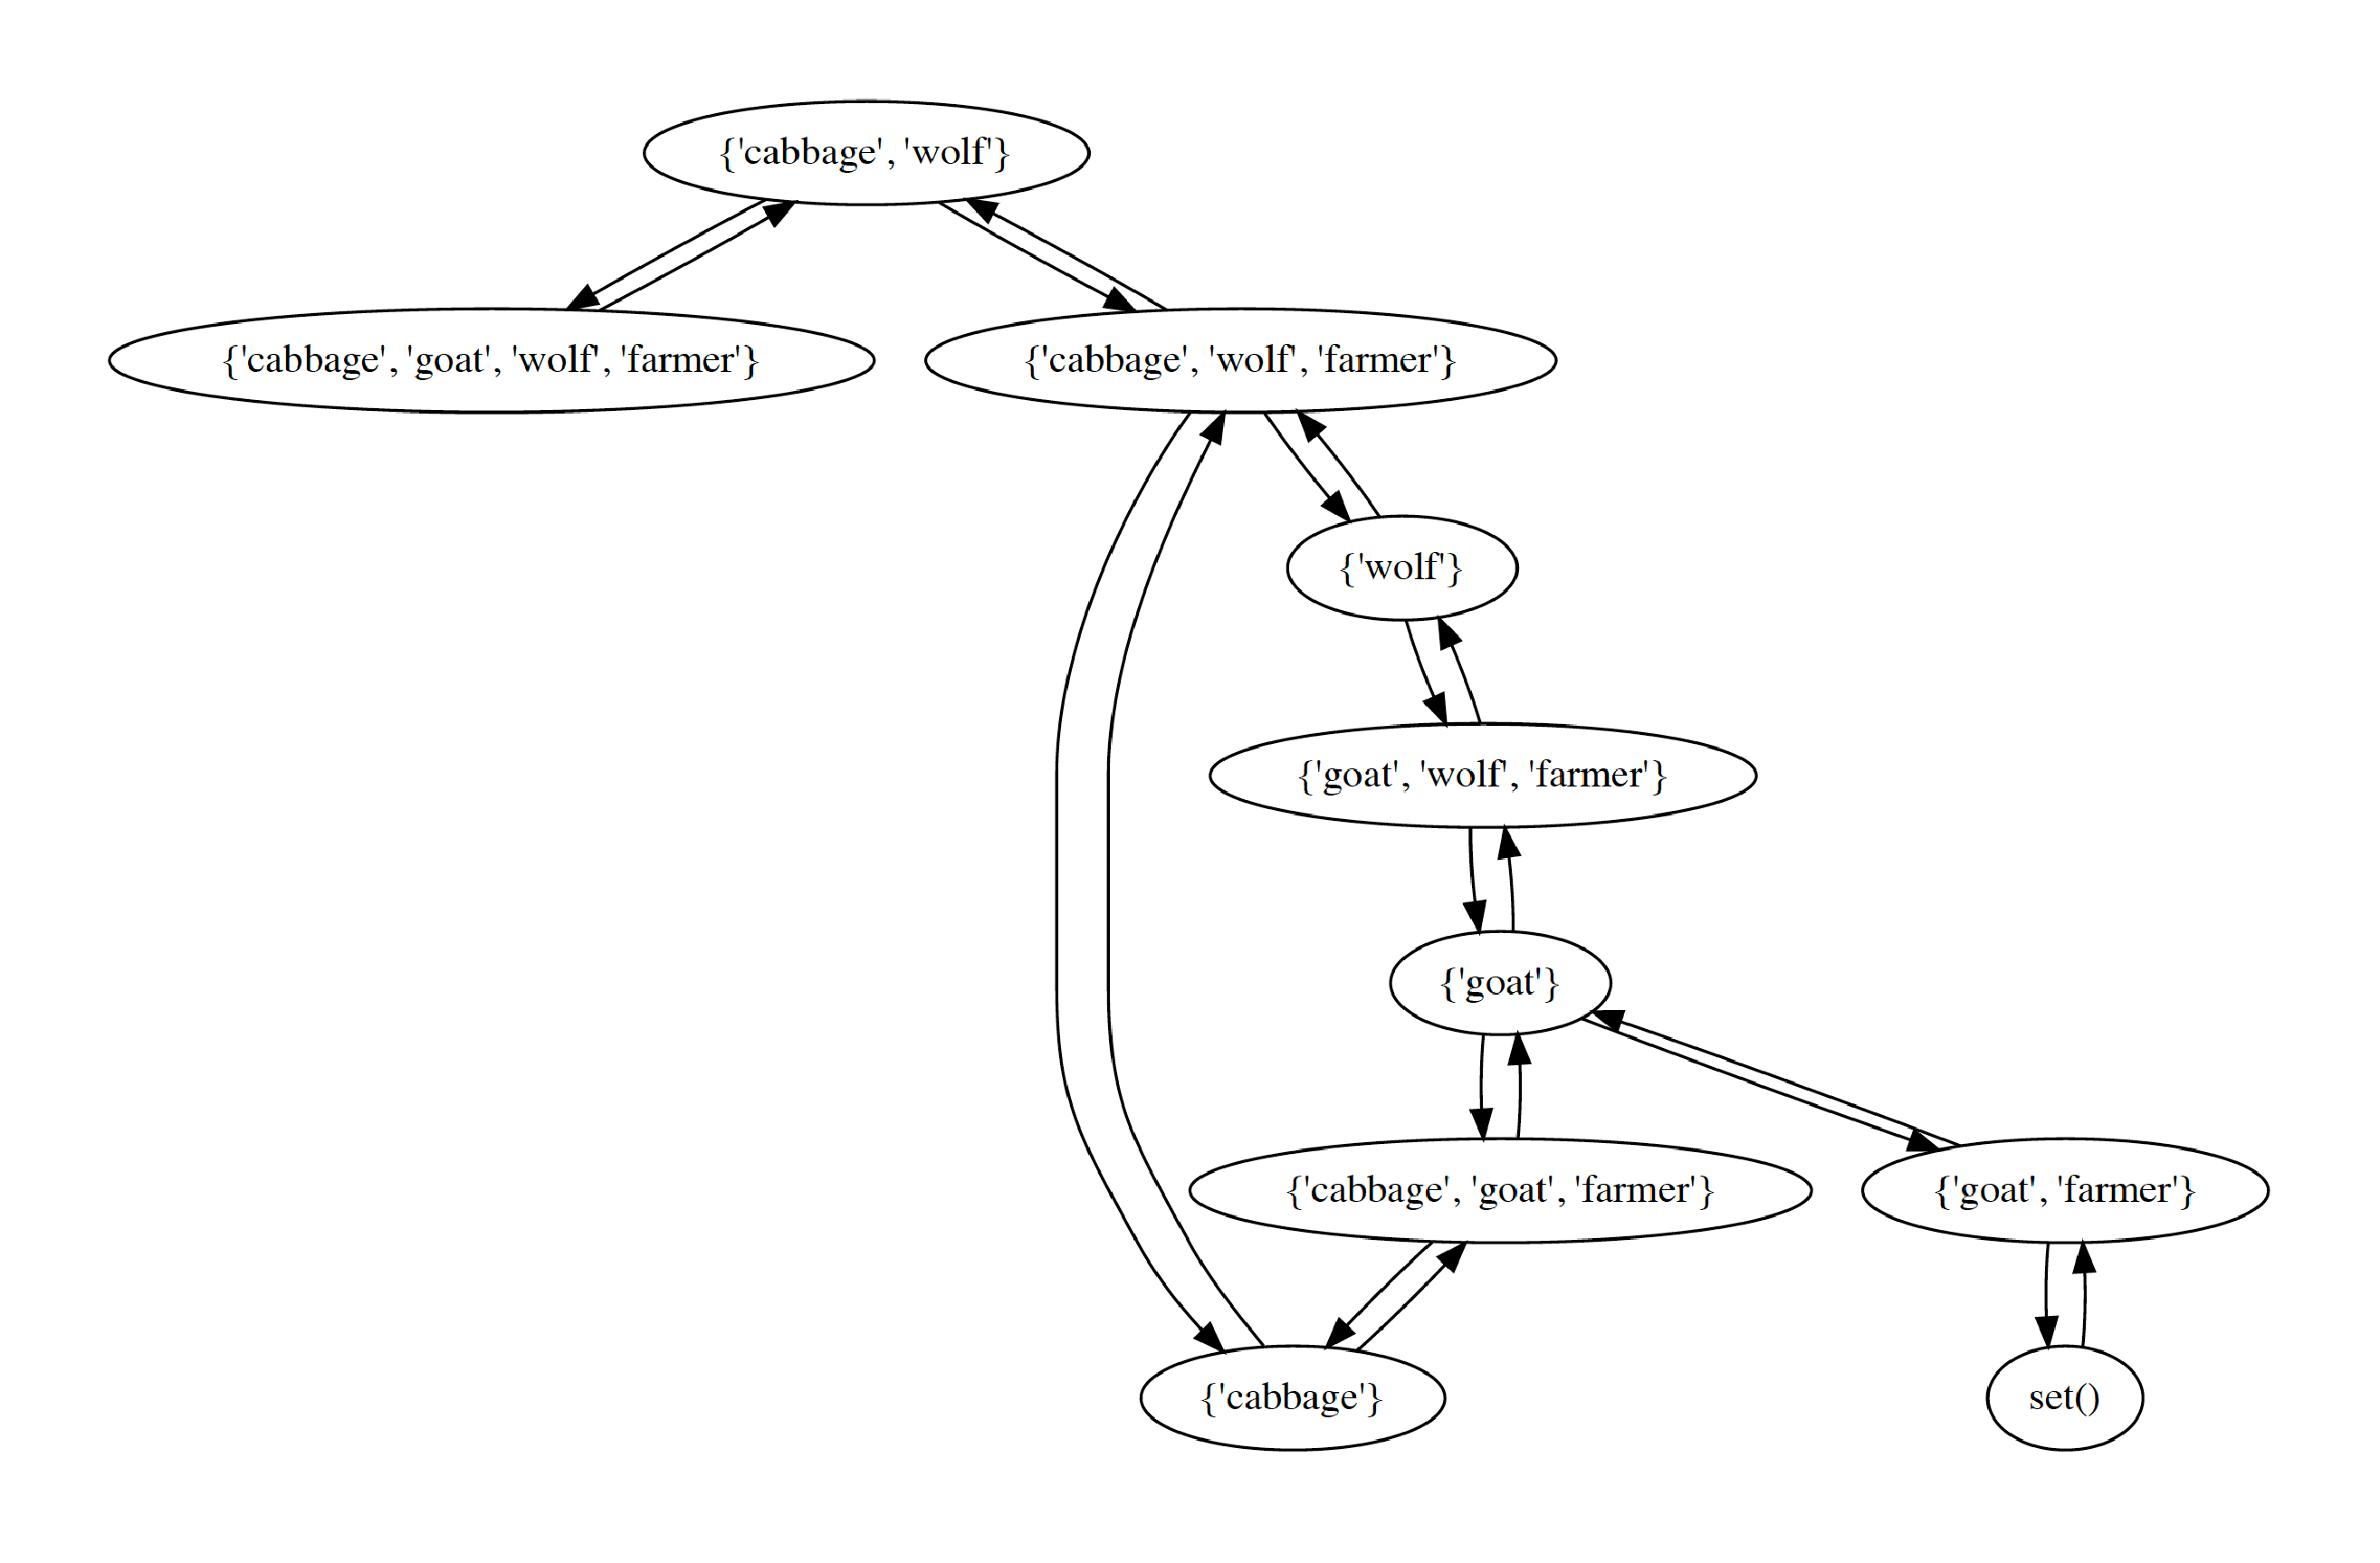
\epsfig{file=Figures/wolf-goat-cabbage, scale=0.4}

  \caption{The relation \texttt{R} shown as a directed graph.}
  \label{fig:wolf-goat-cabbage.pdf}
\end{figure}




Figure \ref{fig:wolf-ziege} on page \pageref{fig:wolf-ziege} shows the program
\href{https://github.com/karlstroetmann/Logik/blob/master/Python/wolf-goat-cabbage.py}{\texttt{wolf-goat-cabbage.py}}
that combines the statements shown so far.  The solution computed by this program is shown in Figure
 \ref{fig:wolf-ziege-solution}.

\begin{figure}[!ht]
  \centering
\begin{Verbatim}[ codes         = {\catcode`$=3\catcode`_=8\catcode`^=7},
                  frame         = lines, 
                  framesep      = 0.3cm, 
                  labelposition = bottomline,
                  numbers       = left,
                  numbersep     = -0.2cm,
                  xleftmargin   = 0.3cm,
                  xrightmargin  = 0.3cm,
                ]
    def problem(S):
        return ('farmer' not in S) and             \
               (('goat' in S and 'cabbage' in S) or   # goat eats cabbage
                ('wolf' in S and 'goat'    in S)   )  # wolf eats goat
    
    All   = frozenset( ['farmer', 'wolf', 'goat', 'cabbage'] )
    R1    = { (S, S - B) for S in States for B in power(S)
                         if S - B in States and 'farmer' in B and len(B) <= 2
            }
    R2    = { (S2, S1) for (S1, S2) in R1 }
    R     = R1.union(R2)
    start = All
    goal  = frozenset()
    Path  = findPath(start, goal, R)
\end{Verbatim} 
\vspace*{-0.3cm}
\caption{Solving the wolf-goat-cabbage problem.}  
\label{fig:wolf-ziege}
\end{figure}


\begin{figure}[!ht]
  \centering
\begin{Verbatim}[ codes         = {\catcode`$=3\catcode`_=8\catcode`^=7},
                  frame         = lines, 
                  framesep      = 0.3cm, 
                  labelposition = bottomline,
                  numbers       = left,
                  numbersep     = -0.2cm,
                  xleftmargin   = 0.8cm,
                  xrightmargin  = 0.8cm,
                ]
    {"cabbage", "farmer", "goat", "wolf"}                                 {}
                             >>>> {"farmer", "goat"} >>>> 
    {"cabbage", "wolf"}                                   {"farmer", "goat"}
                             <<<< {"farmer"} <<<< 
    {"cabbage", "farmer", "wolf"}                                   {"goat"}
                             >>>> {"farmer", "wolf"} >>>> 
    {"cabbage"}                                   {"farmer", "goat", "wolf"}
                             <<<< {"farmer", "goat"} <<<< 
    {"cabbage", "farmer", "goat"}                                   {"wolf"}
                             >>>> {"cabbage", "farmer"} >>>> 
    {"goat"}                                   {"cabbage", "farmer", "wolf"}
                             <<<< {"farmer"} <<<< 
    {"farmer", "goat"}                                   {"cabbage", "wolf"}
                             >>>> {"farmer", "goat"} >>>> 
    {}                                 {"cabbage", "farmer", "goat", "wolf"}
\end{Verbatim} 
\vspace*{-0.3cm}
\caption{A schedule for the agricultural economist.}  
\label{fig:wolf-ziege-solution}
\end{figure}




\section{Terms and Matching}
So far we have seen the basic data structures of \setlx\ like numbers, string, sets, and lists.
There is one more data structure that is supported by \setlx.  This is the data structure of
\colorbox{amethyst}{\blue{terms}}.  
This data structure is especially useful when we develop programs that deal with mathematical formulas.
For example, in this section we will develop a program that reads a string like 
\\[0.2cm]
\hspace*{1.3cm}
``\texttt{x * exp(x)}'',
\\[0.2cm]
interprets this string as describing the real valued function 
\\[0.2cm]
\hspace*{1.3cm}
$x \mapsto x \cdot \exp(x)$, 
\\[0.2cm]
and then takes the derivative of this function with respect to the variable $x$.  This program is
easy to implement if real valued functions are represented as terms.  The reason is that \setlx\ provides 
\colorbox{amethyst}{\blue{matching}} for terms.  We will define this notion later.  Matching
is one of the main ingredients of the programming language \href{https://en.wikipedia.org/wiki/Prolog}{Prolog}.
This programming language was quite popular in artificial intelligence during the eighties and has
inspired the matching that is available in \textsl{Python}.


\subsection{Constructing and Manipulating Terms}
In order to build terms, we first need \colorbox{amethyst}{\blue{functors}}.  It is important not to confuse functors with
function symbols.  Therefore, functors have to be preceded by the character  
``\texttt{@}''.
For example, the following strings can be used as functors:
\\[0.2cm]
\hspace*{1.3cm}
\texttt{@f}, \quad \texttt{@FabcXYZ}, \quad \texttt{@sum}, \quad \texttt{@Hugo\_}.
\\[0.2cm]
However, in the expression ``\texttt{@f}'', the string ``\texttt{f}'' is the functor.  The
character ``\texttt{@}'' is only used as an escape character that tells us that ``\texttt{f}'' is
not a function symbol but rather a functor.  Next, we define \colorbox{amethyst}{\blue{terms}}.  If $F$ is a functor and 
$t_1$, $t_2$, $\cdots$, are any values, i.e.~they could be number, strings, lists, sets, or terms
themselves, then
\\[0.2cm]
\hspace*{1.3cm}
$\texttt{@}F(t_1, t_2, \cdots, t_n)$
\\[0.2cm]
is a term.  Syntactically, terms look very similar to function calls.  The only difference between a function call
and a term is the following: 
\begin{enumerate}
\item A function call starts with a function symbol. 
\item A term starts with a functor. 
\end{enumerate}


\examplesEng
\begin{enumerate}
\item \texttt{@Address(\symbol{39}Coblitzallee 1-9\symbol{39}, 68163, \symbol{39}Mannheim\symbol{39})}

      is a term that represents an address.
\item \texttt{@product(@variable(\symbol{39}x\symbol{39}), @exp(@variable(\symbol{39}x\symbol{39})))}

      is a term that represents the  function $x \mapsto x \cdot \exp(x)$.  
      \eox
\end{enumerate}
At this point you might ask how terms are evaluated.  The answer is that terms
\colorbox{amethyst}{are not evaluated!}  
Terms are used to represent data in a way that is both concise and readable.  Hence, terms are values like
numbers, sets or strings.  As terms are values, they don't need to be evaluated.

Let us demonstrate a very simple application of terms.  Imagine that \setlx\ wouldn't provide lists as a native data
type.  Then, we could implement lists via terms.  First, we would use a functor to represent the empty list.
Let us choose the functor \texttt{nil} for this purpose.  Hence, we have
\\[0.2cm]
\hspace*{1.3cm}
$\texttt{@nil()} \;\widehat{=}\; \texttt{[]}$,
\\[0.2cm]
where we read the symbol ``$\widehat{=}$'' as ``corresponds to''.
Note that the parentheses after the functor  \texttt{nil} are \colorbox{amethyst}{necessary!}  Next, in order to represent
a list with first element $x$ and a list $r$ of remaining elements we use the functor \texttt{cons}.
Then we have the correspondence
\\[0.2cm]
\hspace*{1.3cm}
$\texttt{@cons}(x, r) \;\widehat{=}\; \texttt{[}x\texttt{]} + r$. 
\\[0.2cm]
Concretely, the list \texttt{[1,2,3]} is represented as the term
\\[0.2cm]
\hspace*{1.3cm}
\texttt{@cons(1, @cons(2, @cons(3, @nil())))}.
\\[0.2cm]
The programming language \textsl{Prolog} represents lists internally in a similar form.

\setlx\ provides two functions that allow us to extract the components of a term.  Furthermore, there is a
function for constructing terms.  These functions are described next.
\begin{enumerate}
\item The function \texttt{fct} returns the functor of a given term.
      If  $t$ is a term of the form $\at F(s_1,\cdots,s_n)$, then the result returned by the expression
      \\[0.2cm]
      \hspace*{1.3cm}
      $\texttt{fct}(\at F(s_1,\cdots,s_n))$
      \\[0.2cm]
      is the functor $F$ of this term.  For example the expression
      \\[0.2cm]
      \hspace*{1.3cm}
      \texttt{fct(@cons(1, @cons(2, @cons(3, @nil()))))}
      \\[0.2cm]
      returns the string  \texttt{\symbol{39}cons\symbol{39}} as its result.
\item The function \texttt{args} returns the arguments of a term.
      If  $t$ is a term of the form $\at F(s_1,\cdots,s_n)$, then
      \\[0.2cm]
      \hspace*{1.3cm}
      $\mathtt{args}(\at F(s_1,\cdots,s_n))$
      \\[0.2cm]
      returns the list $[s_1, \cdots, s_n]$. For example, the expression
      \\[0.2cm]
      \hspace*{1.3cm}
      \texttt{args(\at cons(1, \at cons(2, \at cons(3, \at nil()))))}
      \\[0.2cm]
      is evaluated as
      \\[0.2cm]
      \hspace*{1.3cm}
      \texttt{[1, \at cons(2, \at cons(3, \at nil()))]}.
\item If $f$ is the name of a functor and  $l$ is a list, then the function \texttt{makeTerm} can be invoked as
      \\[0.2cm]
      \hspace*{1.3cm}
      $t \;\mathtt{=}\; \texttt{makeTerm}(f,l)$.
      \\[0.2cm]
      This expression generates a term $t$ such that $f$ is the functor and $l$ is the list of its
      arguments.  Therefore we have
      \\[0.2cm]
      \hspace*{1.3cm}
      $\mathtt{fct}(t) = f$  \quad und \quad $\mathtt{args}(t) = l$.
      \\[0.2cm]
      For example, the expression
      \\[0.2cm]
      \hspace*{1.3cm}
      \texttt{makeTerm(\symbol{39}cons\symbol{39}, [ 1, \at nil() ])}
      \\[0.2cm]
      returns the result
      \\[0.2cm]
      \hspace*{1.3cm}
      \texttt{\at cons(1, \at nil())}.
\end{enumerate}

\begin{figure}[!ht]
\centering
\begin{Verbatim}[ frame         = lines, 
                  framesep      = 0.3cm, 
                  firstnumber   = 1,
                  labelposition = bottomline,
                  numbers       = left,
                  numbersep     = -0.2cm,
                  xleftmargin   = 0.8cm,
                  xrightmargin  = 0.8cm,
                ]
    append = procedure(l, x) {
        if (fct(l) == "nil") {
            return @cons(x, @nil());  
        }
        [head, tail] = args(l);
        return @cons(head, append(tail, x));
    };
    l = @cons(1, @cons(2, @cons(3, @nil()))); // corresponds to [1,2,3]
    print(append(l, 4));
\end{Verbatim}
\vspace*{-0.3cm}
\caption{Appending an element at the end of a list.}
\label{fig:append.py}
\end{figure}

Figure \ref{fig:append.py} on page \pageref{fig:append.py} shows the
program \href{https://github.com/karlstroetmann/Logik/blob/master/Python/append.py}{\texttt{append.py}}.
This program implements the function \texttt{append}.  As its first arguments, this function takes a list \texttt{l}
that is represented as a term.  As its second argument,  it takes an object \texttt{x}.  The purpose of the expression
\\[0.2cm]
\hspace*{1.3cm}
$\texttt{append}(\texttt{l}, \texttt{x})$
\\[0.2cm]
is to append the object \texttt{x} at the end of the list \texttt{l}.  The implementation of the function \texttt{append}
assumes that the list \texttt{l} is represented as a term using the functors ``\texttt{cons}'' and ``\texttt{nil}''.
\begin{enumerate}
\item Line 2 checks whether the list  \texttt{l} is empty. The list \texttt{l} is empty iff we have
      $\texttt{l} = \texttt{\at nil()}$.  In the program we merely check the functor of the term \texttt{l}.  If the name of this functor is
      \texttt{\symbol{39}nil\symbol{39}}, then \texttt{l} is the empty list.
\item If \texttt{l} is not empty, then it must be a term of the form
      \\[0.2cm]
      \hspace*{1.3cm}
      $\texttt{l} = \texttt{\at cons(\textsl{head}, \textsl{tail})}$.
      \\[0.2cm]     
      Then, conceptually \texttt{head} is the first element of the list \texttt{l} and \texttt{tail} is the list of
      the remaining elements.  In this case, we need to recursively append \texttt{t} at the end of the list \texttt{tail}.
      Finally, the first element of the list \texttt{l}, which is called \texttt{head} in line 5, needs
      to be prepended to the list that is returned from the recursive invocation of \texttt{append}.
      This is done in line 6 by constructing the term 
      \\[0.2cm]
      \hspace*{1.3cm}
      \texttt{@cons(head, append(tail, x))}.
\end{enumerate}

\subsection{Matching}
It would be quite tedious if the functions \texttt{fct} and \texttt{args} were the only means to extract the
components of a term.  Figure \ref{fig:append-match.py} on page \pageref{fig:append-match.py}
shows the program
\href{https://github.com/karlstroetmann/Logik/blob/master/Python/append-match.py}{\texttt{append-match.py}}, 
that uses \blue{matching} to implement the function \texttt{append}.  
Line 3 checks, whether the list  \texttt{l} is empty, i.e.~whether \texttt{l} is identical to the term 
\texttt{@nil()}.  Line 4 is more interesting, as it combines two actions.
\begin{enumerate}
\item It checks, whether the list \texttt{l} is a term that starts with the functor \texttt{cons}.
\item If \texttt{l} does indeed starts with the functor \texttt{cons}, the arguments of this functor are
      extracted and assigned to the variables \texttt{head} and \texttt{tail}.
\end{enumerate}
Hence, if the \texttt{match} statement in line 4 is successful, the equation
\\[0.2cm]
\hspace*{1.3cm}
$\texttt{l} = \texttt{@cons(head, tail)}$
\\[0.2cm]
holds afterwards.


\begin{figure}[!ht]
\centering
\begin{Verbatim}[ frame         = lines, 
                  framesep      = 0.3cm, 
                  firstnumber   = 1,
                  labelposition = bottomline,
                  numbers       = left,
                  numbersep     = -0.2cm,
                  xleftmargin   = 0.8cm,
                  xrightmargin  = 0.8cm,
                ]
    append = procedure(l, x) {
        match (l) {
            case @nil():            return @cons(x, @nil());
            case @cons(head, tail): return @cons(head, append(tail, x));
        }
    };
\end{Verbatim}
\vspace*{-0.3cm}
\caption{Implementing \texttt{append} using a \texttt{match} statement.}
\label{fig:append-match.py}
\end{figure}
In general, a \texttt{match} statement has the structure that is shown in Figure \ref{fig:match}.
Here, $e$ is any expression that yields a term when evaluated.  The expressions 
$t_1$, $\cdots$, $t_n$ are so called \blue{patterns} that contain variables.  When the \texttt{match} statement
is executed, \textsl{Python} tries to bind the variables occurring in the pattern $t_1$ such that the resulting
expression is equal to $e$.  If this succeeds, the statements in  $\textsl{body}_1$ are executed and the
execution of the \texttt{match} statement ends.
Otherwise, the patterns $t_2$, $\cdots$, $t_n$ are tried one by one.  If the pattern $t_i$ is successfully
matched to $e$, the statements in $\textsl{body}_i$ are executed and the execution of the \texttt{match}
statement end.  If none of the patterns $t_1$, $\cdots$, $t_n$ can be matched with $e$, the statements in
$\textsl{body}_{n+1}$ are executed.


\begin{figure}[!ht]
  \centering
\begin{Verbatim}[ codes         = {\catcode`_=8\catcode`^=7},
                  frame         = lines, 
                  framesep      = 0.3cm, 
                  labelposition = bottomline,
                  numbers       = left,
                  numbersep     = -0.2cm,
                  commandchars  = \\\{\},
                  xleftmargin   = 0.8cm,
                  xrightmargin  = 0.8cm
                ]
      \texttt{\underline{match} (\(e\)) \{}
          \texttt{\underline{case}} \(t_1\) : \textsl{body}\(_1\) 
          \vdots
          \texttt{\underline{case}} \(t_n\) : \textsl{body}\(_n\)
          \texttt{\underline{default}:} \textsl{body}\(_{n+1}\)
      \texttt{\}}
\end{Verbatim}
\vspace*{-0.3cm}
\caption{Struktur eines \texttt{Match}-Blocks}  \label{fig:match}
\end{figure} 


\begin{figure}[!ht]
\centering
\begin{Verbatim}[ frame         = lines, 
                  framesep      = 0.3cm, 
                  firstnumber   = 1,
                  labelposition = bottomline,
                  numbers       = left,
                  numbersep     = -0.2cm,
                  xleftmargin   = 0.8cm,
                  xrightmargin  = 0.8cm,
                ]
    loadLibrary("termUtilities");  

    diff = procedure(t, x) {
        match (t) {
            case a + b :
                return diff(a, x) + diff(b, x);
            case a - b :
                return diff(a, x) - diff(b, x);
            case a * b :
                return diff(a, x) * b + a * diff(b, x);
            case a / b :
                return ( diff(a, x) * b - a * diff(b, x) ) / b * b;
            case a ** b :
                return diff( @exp(b * @ln(a)), x);
            case @ln(a) :
                return diff(a, x) / a;
            case @exp(a) :
                return diff(a, x) * @exp(a);
            case v | v == x :
                return 1;
            case y | isVariable(y) :  // must be different from x
                return 0;
            case n | isNumber(n):   
                return 0;  
         }
    };
    test = procedure(s) {
        t = parseTerm(s);
        v = parseTerm("x");
        d = diff(t, v);
        print("d/dx($s$) = $d$\n");
    };
    test("x ** x");
\end{Verbatim}
\vspace*{-0.3cm}
\caption{A function to perform symbolic differentiation.}
\label{fig:diff.py}
\end{figure}

\noindent
We close this section by showing an example that demonstrates the power of matching.
The function \texttt{diff} that is shown in Figure \ref{fig:diff.py} on page \pageref{fig:diff.py} is part
of the program
\href{https://github.com/karlstroetmann/Logik/blob/master/Python/diff.py}{\texttt{diff.py}}.
This function is called with two arguments.
\begin{enumerate}
\item The first argument \texttt{t} is a term that represents an arithmetical expression.
\item The second argument \texttt{x} is a term that represents a variable.
\end{enumerate}
The function \texttt{diff} interprets its argument \texttt{t} as a function of the variable
\texttt{x}.  We take the \href{https://en.wikipedia.org/wiki/Derivative}{derivative} of this
function with respect to the variable \texttt{x}.  For example, in order to compute the derivative of
the function
\\[0.2cm]
\hspace*{1.3cm}
$x \mapsto x^x$,
\\[0.2cm]
we can call the function  \texttt{diff} as follows:
\\[0.2cm]
\hspace*{1.3cm}
\texttt{diff(parseTerm(\symbol{39}x ** x\symbol{39}), parseTerm(\symbol{39}x\symbol{39}));}
\\[0.2cm]
Here, the function \texttt{parseTerm} is a function that is defined in the library \texttt{termUtilities}.
This function takes a string as input and converts this string into a term.  In order to use the function
\texttt{parseTerm}, we have to load the library that defines it.  This happens in line 1 of Figure
\ref{fig:diff.py}. 

Let us now discuss the implementation of the function \texttt{diff} in more detail.  
\begin{enumerate}
\item Line 5 makes use of the fact that the operator ``\texttt{+}'' can be applied to terms.
      The result is a term that has the functor ``\texttt{@@@sum}''.  However, this functor is hidden from the
      user and becomes only visible when we use the function \texttt{fct} to expose it.  For example, we can
      define a term \texttt{t} as follows:
      \\[0.2cm]
      \hspace*{1.3cm}
      \texttt{t = @f(1) + @g(2);}
      \\[0.2cm]
      Then \texttt{t} is a term that is displayed as ``\texttt{@f(1) + @g(2)}'', but the expression
      \texttt{fct(t)} returns the string
      \\[0.2cm]
      \hspace*{1.3cm}
      \texttt{"@@@sum"}.
      \\[0.2cm]
      There is no need to remember that the internal representation of the operator ``\texttt{+}'' as a functor
      is given as the string ``\texttt{@@@sum}'''.  The only thing that you have to keep in mind is
      the fact, that the operator ``\texttt{+}'' can be applied to terms.  The same is true for the
      other arithmetical operators ``\texttt{+}'', ``\texttt{-}'', ``\texttt{*}'', ``\texttt{/}'',
      ``\texttt{\symbol{37}}'', and ``\texttt{**}''.  Similarly, the logical operators
      ``\texttt{\&\&}'', ``\texttt{||}'', ``\texttt{!}'', ``\texttt{=>}'', and ``\texttt{<==>}'' can
      be used as functors.  Note, however, that the relational operators ``\texttt{<}'',
      ``\texttt{>}'', ``\texttt{<=}'', ``\texttt{>=}'' \colorbox{amethyst}{can not be used} to
      combine terms.  Finally, the operators ``\texttt{==}'' and ``\texttt{!=}'' can be used to
      check whether two terms are identical or different, respectively.  Hence, while these
      operators can be applied to terms, they return a Boolean value, not a term!
      
      As the operator ``\texttt{+}'' can be used as a functor, it can also be used in a pattern.  The
      pattern 
      \\[0.2cm]
      \hspace*{1.3cm}
      \texttt{a + b}
      \\[0.2cm]
      matches any term that can be written as a sum.  The derivative of a sum is computed by summing the
      derivatives of the components of the sum, i.e.~we have
      \\[0.2cm]
      \hspace*{1.3cm}
      $\ds \diff\bigl(f(x) + g(x)\bigr) = \diff f(x) + \diff g(x)$.
      \\[0.2cm]
      Therefore, the case where the term \texttt{t} has the form \texttt{a + b} can be dealt with by
      recursively computing the derivatives of \texttt{a} and \texttt{b} and adding them.  This
      happens in line 6.
\item Line 7 deals with the case where \texttt{t} is a difference.  Mathematically, the rule to take the
      derivative of a difference is
      \\[0.2cm]
      \hspace*{1.3cm}
      $\ds \diff\bigl(f(x) - g(x)\bigr) = \diff f(x) - \diff g(x)$.
      \\[0.2cm]
      This rule is implemented in line 8.
\item Line 9 deals with the case where \texttt{t} is a product.  The 
      \href{https://en.wikipedia.org/wiki/Product_rule}{product rule} is
      \\[0.2cm]
      \hspace*{1.3cm}
      $\ds \diff\bigl(f(x) \cdot g(x)\bigr) = \left(\diff f(x)\right)\cdot g(x) + f(x) \cdot \left(\diff g(x)\right)$.
      \\[0.2cm]
      This rule is implemented in line 10.
\item Line 11 deals with the case where \texttt{t} is a quotient.  The
      \href{https://en.wikipedia.org/wiki/Quotient_rule}{quotient rule} is 
      \\[0.2cm]
      \hspace*{1.3cm}
      $\ds \diff\left(\frac{f(x)}{g(x)}\right) = \frac{\left(\diff f(x)\right)\cdot g(x) - f(x)
        \cdot \left(\diff g(x)\right)}{g(x) \cdot g(x)}$.
      \\[0.2cm]
      This rule is implemented in line 12.
\item Line 13 deals with the case where \texttt{t} is a power.  Now in order to take the derivative of an
      expression of the form
      \\[0.2cm]
      \hspace*{1.3cm}
      $\ds f(x)^{g(x)}$
      \\[0.2cm]
      we first need to rewrite it using the following trick:
      \\[0.2cm]
      \hspace*{1.3cm}
      $\ds f(x)^{g(x)} = \exp\bigl(\ln\bigl(f(x)^{g(x)}\bigr)\bigr) = \exp\bigl(g(x) \cdot \ln(f(x))\bigr)$,
      \\[0.2cm]
      Then, we can recursively call \texttt{diff} for this expression.  This works, because the function
      \texttt{diff} can deal with both the exponential function $x \mapsto \exp(x)$ and with the natural
      logarithm $x \mapsto \ln(x)$.  This rewriting is done in line 14.
\item Line 15 deals with the case where \texttt{t} has the form $\ln\bigl(f(x)\bigr)$.  
      In order to take the derivative of this expression, we first need to know the derivative of the natural
      logarithm.  This derivative is given as 
      \\[0.2cm]
      \hspace*{1.3cm}
      $\ds \diff \ln(x) = \frac{1}{x}$.
      \\[0.2cm]
      Then, using the \href{https://en.wikipedia.org/wiki/Chain_rule}{chain rule} we have that
      \\[0.2cm]
      \hspace*{1.3cm}
      $\ds \diff \ln\bigl(f(x)\bigr) = \frac{\diff f(x)}{f(x)}$.
      \\[0.2cm]
      This rule is used in line 16.
\item Line 17 deals with the case where \texttt{t} has the form $\exp\bigl(f(x)\bigr)$.  
      In order to take the derivative of this expression, we first need to know the derivative of the 
      \href{https://en.wikipedia.org/wiki/Exponential_function}{exponential function}.  This derivative is given as 
      \\[0.2cm]
      \hspace*{1.3cm}
      $\ds \diff \exp(x) = \exp(x)$.
      \\[0.2cm]
      Then, using the \href{https://en.wikipedia.org/wiki/Chain_rule}{chain rule} we have that
      \\[0.2cm]
      \hspace*{1.3cm}
      $\ds \diff \exp\bigl(f(x)\bigr) = \left(\diff f(x)\right) \cdot \exp\bigl(f(x)\bigr)$.
      \\[0.2cm]
      This rule is used in line 18.
\item Line 19 deals with the case where \texttt{t} is a variable and happens to be the same variable as
      \texttt{x}.  This is checked using the condition
      \\[0.2cm]
      \hspace*{1.3cm}
      \texttt{v == x}
      \\[0.2cm]
      that is attached using the \blue{condition operator} ``\texttt{|}''.   Since we have
      \\[0.2cm]
      \hspace*{1.3cm}
      $\ds \frac{\mathrm{d}x}{\mathrm{d}x} = 1$,
      \\[0.2cm]
      the function \texttt{diff} returns \texttt{1} in this case.
\item Line 21 deals with the case where \texttt{t} is a variable.  As line 19 has already covered the case that
      \texttt{t} and \texttt{x} are the same variable, in this case the variable \texttt{x} must be different
      from \texttt{t}.  Therefore, with respect to \texttt{x} the term \texttt{t} can be seen as a constant and
      the derivative is \texttt{0}.
\item Line 23 covers the case where \texttt{t} is a number.  Note how we call \texttt{isNumber}
      after the condition operator ``\texttt{|}''.  As a number is a constant, the derivative is \texttt{0}.
\item Line 27 defines the procedure \texttt{test}.  This procedure takes a string \texttt{s} and transforms it
      into the term \texttt{t} via the function \texttt{parseTerm} defined in the library
      \texttt{termUtilities}.  Similarly, the string \texttt{"x"} is transformed into the term \texttt{v} that
      represents this variable.\footnote{Internally, this variable is represented as the term
      ``\texttt{@@@variable("x")}''.}
      Line 30 call the function \texttt{diff} using the term \texttt{t} and the variable \texttt{v}
      as arguments.  The resulting term is printed in line 31.
\item Line 33 shows how the function \texttt{test} can be called to compute the derivative $\diff x^x$.
\end{enumerate}


\section{Outlook}
This introductory chapter covers only a small part of the programming language  \textsl{Python}.  There are some
additional features of \setlx\ that will be discussed in the following chapters as we need them.
Furthermore,  \textsl{Python} is discussed in depth in the tutorial that can be found at the following address:
\\[0.2cm]
\hspace*{1.3cm}
\href{http://download.randoom.org/setlX/tutorial.pdf}{\texttt{http://download.randoom.org/setlX/tutorial.pdf}}


\remarkEng
Most of the algorithm that were presented in this chapter are not very efficient.  The main purpose of these
algorithms is to serve as examples that were presented for two reasons:
\begin{enumerate}
\item My first intention was to make the abstract notions introduced in set theory more accessible.  For
      example, the program to compute the transitive closure serves to illustrate both the notion of the
      relational product and the transitive closure.  Furthermore, it shows how these notions are useful in
      solving real world problems.
\item Second, these programs serve to introduce the programming language \setlx.
\end{enumerate}
Later, the lecture on
\href{https://github.com/karlstroetmann/Algorithms/blob/master/Lecture-Notes/algorithms.pdf}{algorithms}
will show how to develop efficient algorithms that are more efficient.
\vspace*{0.3cm}


\section{Reflection}
After having completed this chapter, you should be able to answer the following questions.
\begin{enumerate}
\item Which data types are supported in \textsl{Python}?
\item What are the different methods to define a set in \textsl{Python}?
\item Do you understand how to construct lists via iterator? 
\item How can lists be defined in \textsl{Python}?
\item How does \textsl{Python} support binary relations?
\item How does list slicing and list indexing work?
\item How does \textsl{Python} support terms?
\item How does a fixed-point algorithm work?
\item What type of control structures are supported in \textsl{Python}?
\item How can terms be defined and how does matching for terms work?
\end{enumerate}

%%% Local Variables:
%%% mode: latex
%%% TeX-master: "logic"
%%% End:
